\documentclass{beamer}
\usepackage{xcolor}
\usepackage{mathtools}
\usetheme[titlepagelogo=firenze,% Logo for the first page
		  language=italian,
		  bullet=circle,
		  color=blue,
         ]{TorinoTh}
\usepackage[beamer,customcolors]{hf-tikz}
\definecolor{UniBlue}{RGB}{83,121,170}
\setbeamercolor{block title}{use=structure,fg=white,bg=UniBlue}
\setbeamercolor{block body}{use=structure,fg=black,bg=white}

\newcommand*{\bfrac}[2]{\genfrac{}{}{0pt}{1}{#1}{#2}}

\author{}
\rel{{\normalsize \emph{Visual and Multimedia Recognition}}\\\vspace{0.3cm}Lorenzo Cioni}
\title{\huge Improving WATSS web application with Computer Vision techniques}
\date{}

\begin{document}

\titlepageframe

\begin{tframe}{Introduction}

WATSS, \textbf{Web Annotation Tool for Surveillance Scenarios}, is a web-based annotation tool developed to annotate dataset in surveillance systems.

\vspace{0.3cm}

\textbf{Main goal}: improve WATSS with some \textbf{Computer Vision approaches}, in order to make easy for users to use this tool and make the annotation process more \emph{automatic}

\begin{figure}[h]
\begin{center}
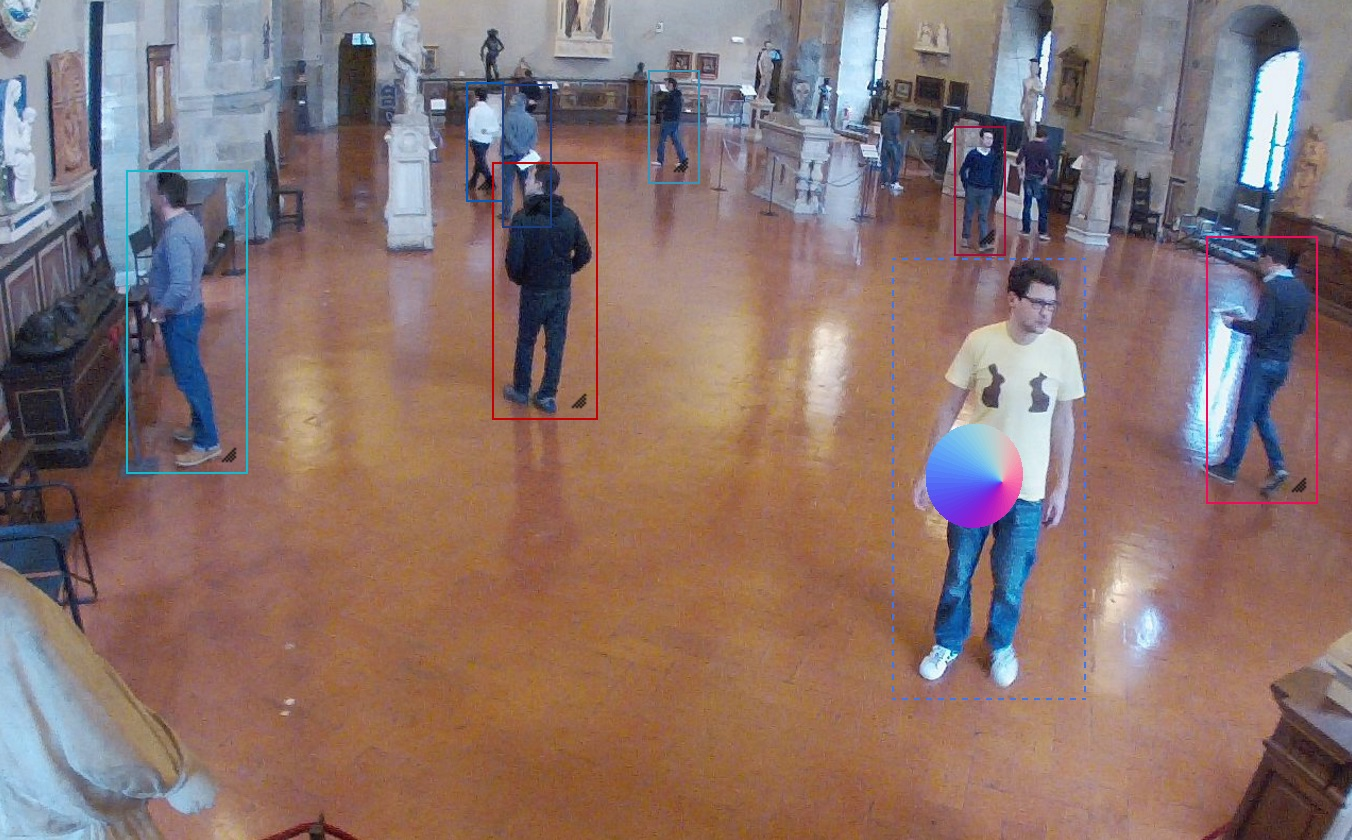
\includegraphics[width=0.4\textwidth]{images/frame.jpg}
\end{center}
\label{fig:mainframe}
\end{figure}

\end{tframe}

\begin{tframe}{Comparative analysis of annotation tools}
\textbf{LabelMe} 
\begin{columns}[t] % align columns
\begin{column}{.5\textwidth}
\begin{itemize}
\item \textbf{Web-based} tool, also for mobile applications
\vspace{0.2cm}
\item Annotate scenes with \textbf{polygonal areas}
\vspace{0.2cm}
\item \textbf{Nested} objects and \textbf{occlusion} annotation
\vspace{0.2cm}
\item \emph{Zoom in} and \emph{out} of the scene
\end{itemize}
\end{column}%
\begin{column}{.3\textwidth}
\begin{figure}[h]
\centering
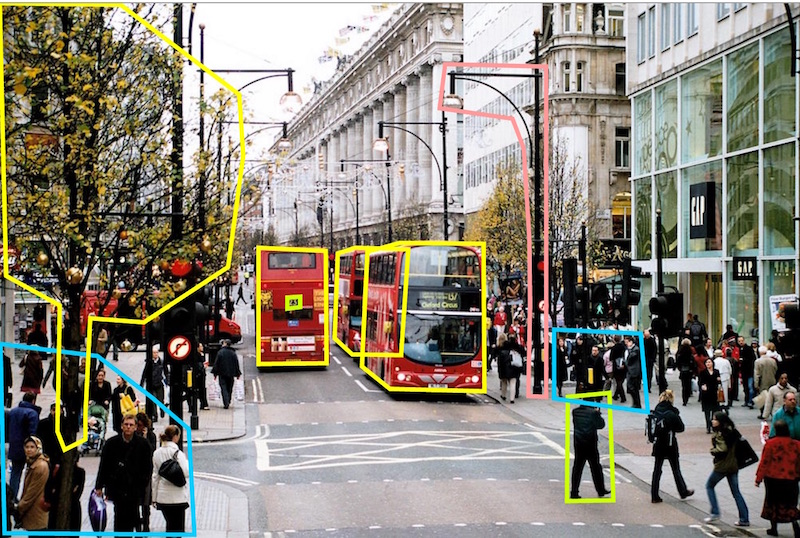
\includegraphics[scale=0.15]{images/labelme.jpg}
\end{figure}
\end{column}%
\end{columns}
\end{tframe}


\begin{tframe}{Comparative analysis of annotation tools}
\textbf{ViPER-GT} 
\begin{columns}[t] % align columns
\begin{column}{.5\textwidth}
\begin{itemize}
\item \textbf{Java application} tool
\vspace{0.2cm}
\item Annotate scenes with \textbf{geometrical shapes}
\vspace{0.2cm}
\item \textbf{Timeline} and \textbf{annotation highlighting} on time change
\vspace{0.2cm}
\item Linear \textbf{interpolation} between annotations
\vspace{0.2cm}
\item \emph{Zoom in} and \emph{out} of the scene
\end{itemize}
\end{column}%
\begin{column}{.3\textwidth}
\begin{figure}[h]
\centering
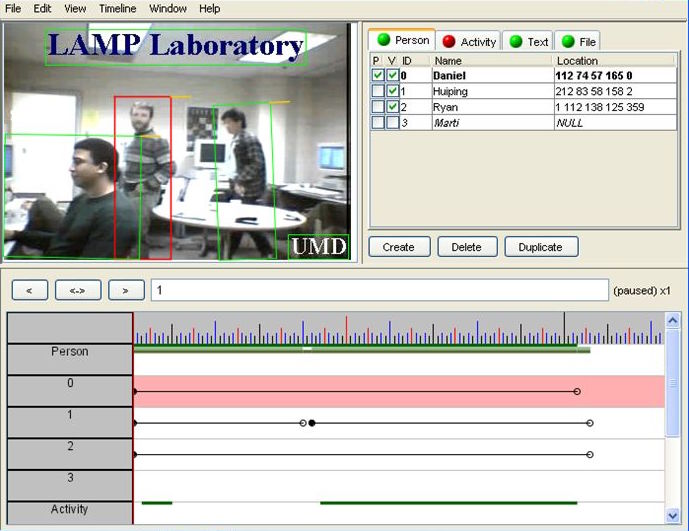
\includegraphics[scale=0.15]{images/vipergt.jpg}
\end{figure}
\end{column}%
\end{columns}
\end{tframe}

\begin{tframe}{Comparative analysis of annotation tools}
\textbf{VATIC} 
\begin{columns}[t] % align columns
\begin{column}{.45\textwidth}
\begin{itemize}
\item \textbf{Online} tool
\vspace{0.1cm}
\item Developed for \textbf{object detection}
\vspace{0.1cm}
\item \textbf{Crowd-sourcing} to Amazon's \emph{Mechanical Turk}
\vspace{0.1cm}
\item Multiple \textbf{plugins}: \emph{object tracking}, \emph{sentence annotation}, etc.
\end{itemize}
\end{column}%
\begin{column}{.3\textwidth}
\begin{figure}[h]
\centering
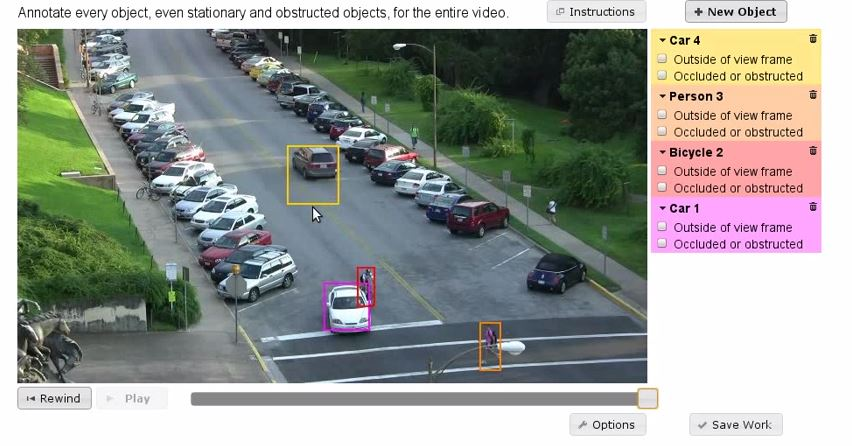
\includegraphics[scale=0.2]{images/vatic.jpg}
\end{figure}
\end{column}%
\end{columns}
\end{tframe}

\begin{tframe}{Comparative analysis of annotation tools}
\textbf{WATSS} 
\begin{columns}[t] % align columns
\begin{column}{.45\textwidth}
\begin{itemize}
\item \textbf{Web-based} tool
\vspace{0.1cm}
\item Annotation with bounding box
\vspace{0.1cm}
\item \textbf{Occlusion} area
\vspace{0.1cm}
\item Coarse \textbf{gaze} estimation
\vspace{0.1cm}
\item \textbf{Groups} and POI under observation
\vspace{0.1cm}
\item \textbf{Multiple cameras} manager
\end{itemize}
\end{column}%
\begin{column}{.3\textwidth}
\begin{figure}[h]
\centering
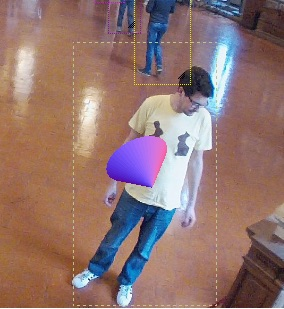
\includegraphics[scale=0.4]{images/gaze.jpg}
\end{figure}
\end{column}%
\end{columns}
\end{tframe}


\begin{tframe}{Improvements}
\begin{itemize}
\vspace{0.3cm}
\item \textbf{User interface} renovation
\vspace{0.2cm}
\item Simpler annotation making and editing
\vspace{0.2cm}
\item Video \textbf{timeline} for annotations
\vspace{0.2cm}
\item Annotation automatic \textbf{proposals} generation
\vspace{0.2cm}
\item \textbf{Scene geometry}-based enhancement
\vspace{0.2cm}
\item Easy \textbf{setup} process
\end{itemize}
\end{tframe}

\begin{tframe}{User interface renovation}
The \textbf{old} WATSS user interface
\begin{figure}[h]
\centering
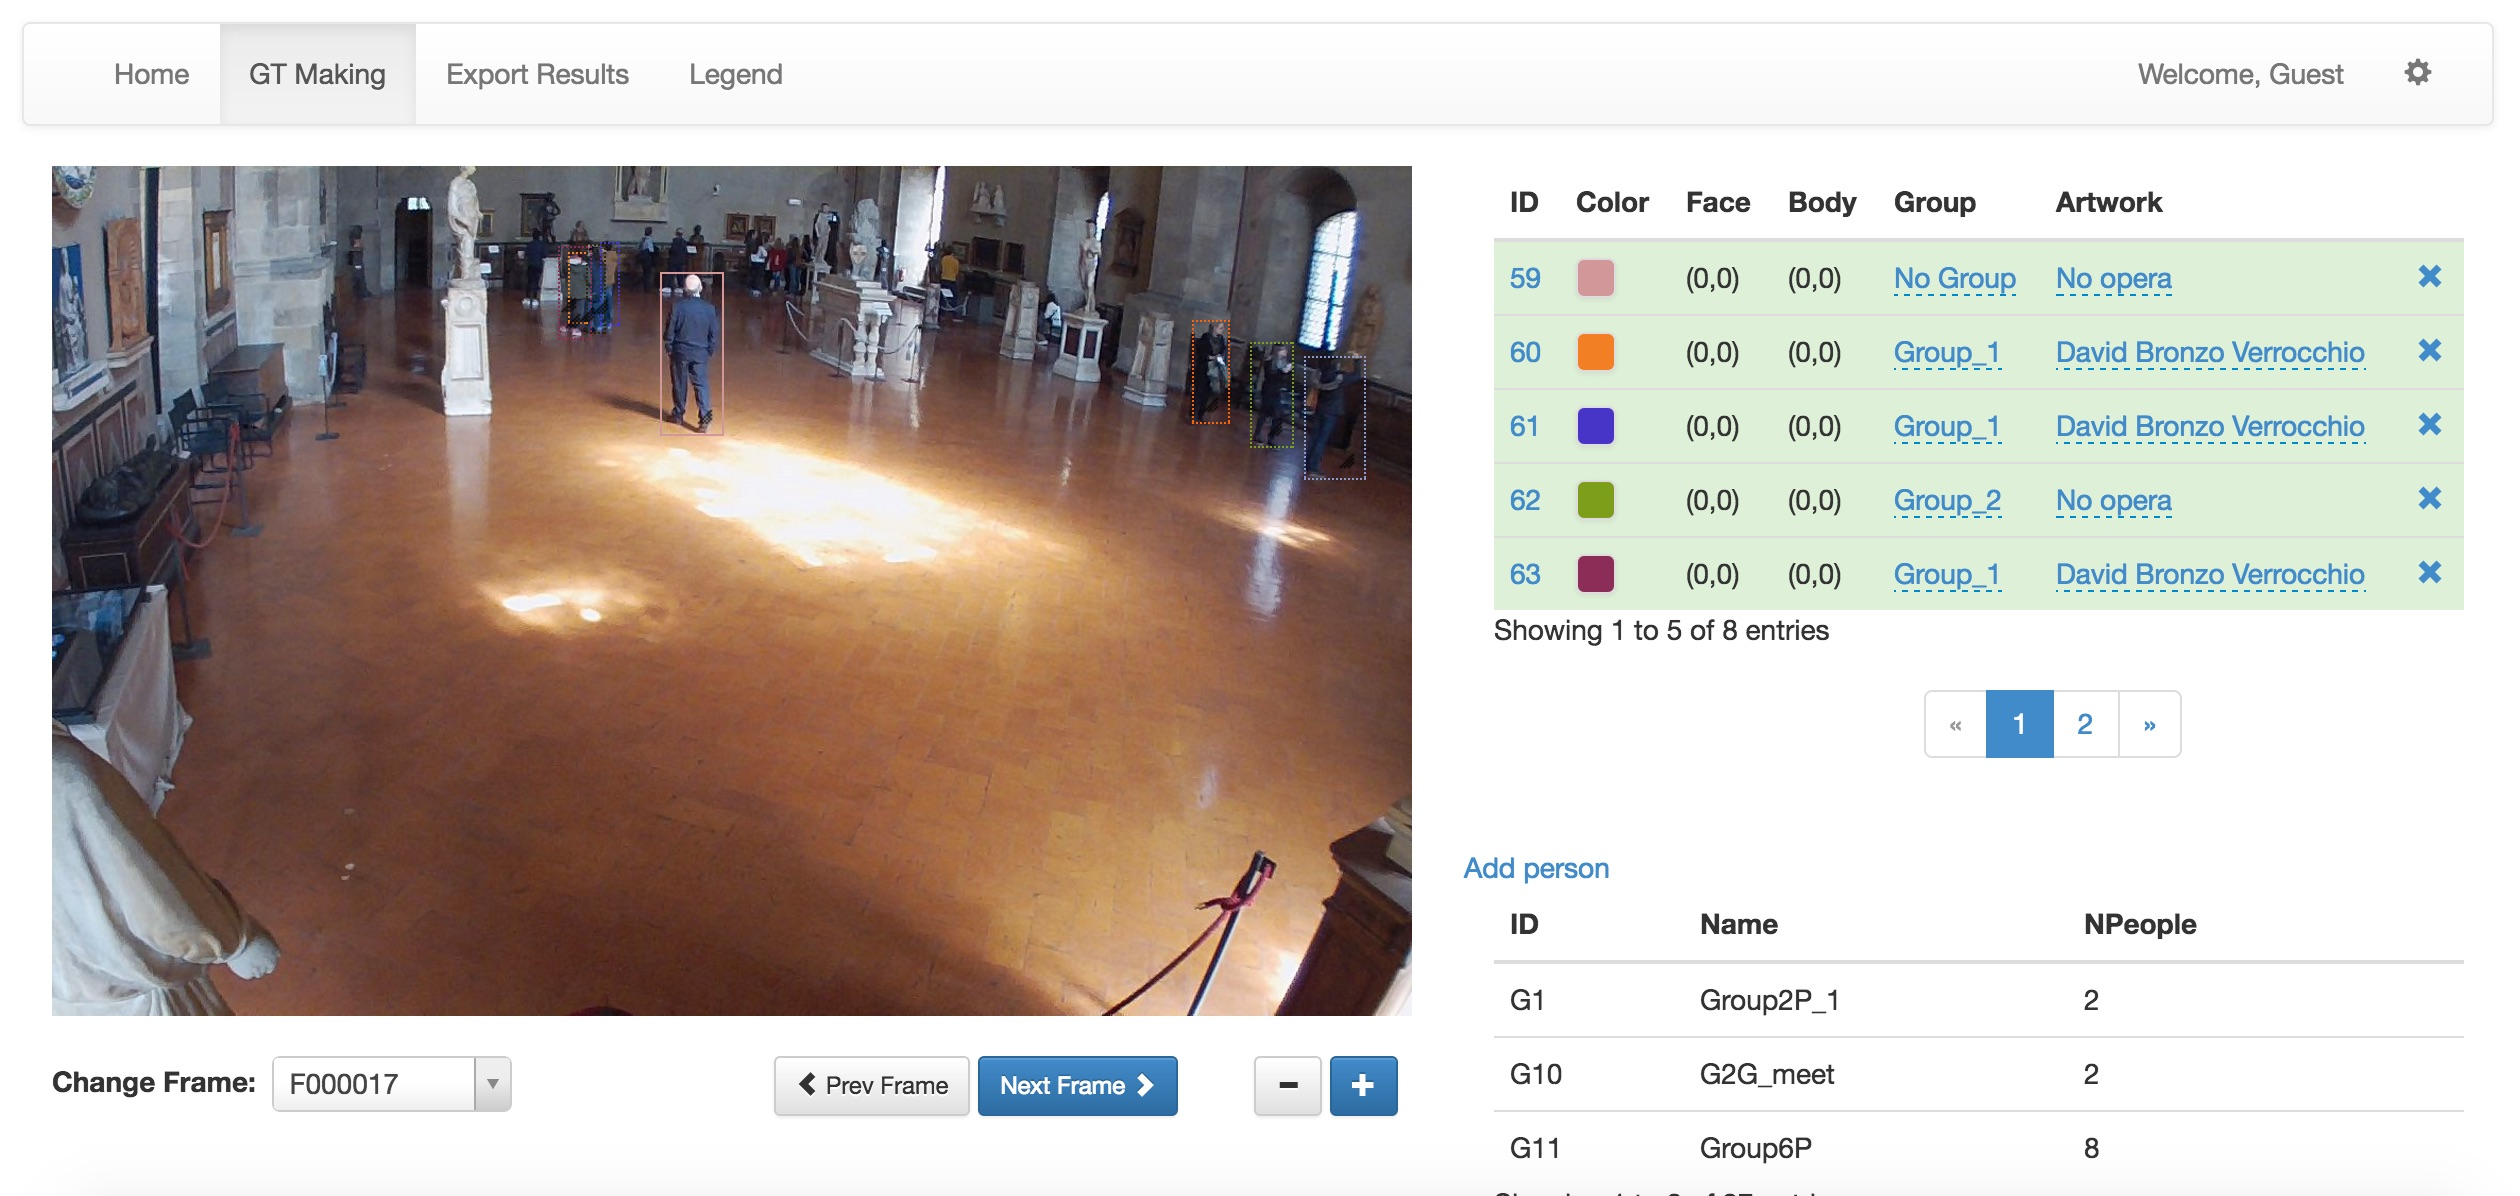
\includegraphics[scale=0.13]{images/watss_old.jpg}
\end{figure}
\end{tframe}

\begin{tframe}{User interface renovation}
The \textbf{new} WATSS user interface
\begin{figure}[h]
\centering
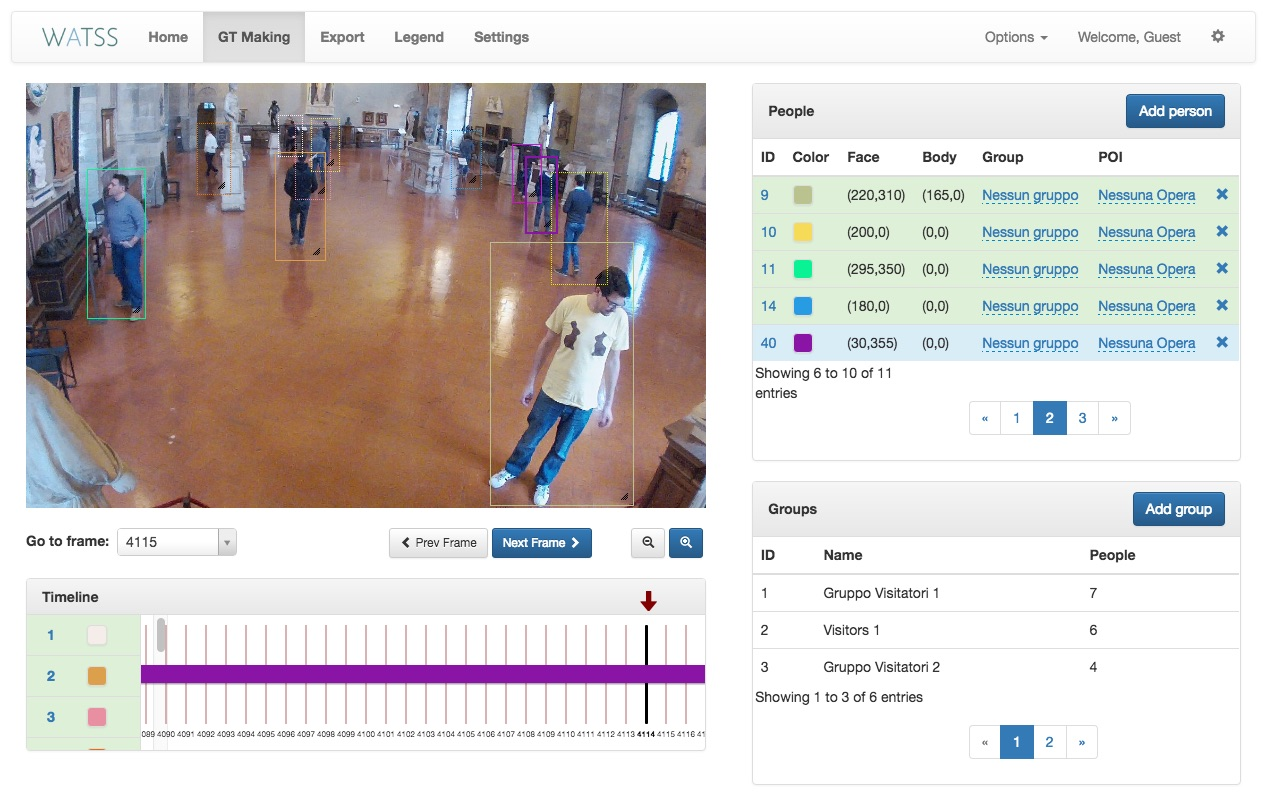
\includegraphics[scale=0.22]{images/watss-gui.jpg}
\end{figure}
\end{tframe}

\begin{tframe}{Video timeline}
In the video \textbf{timeline} all the video frames are shown, coloring the ones with at least one annotated person. 
\vspace{0.2cm}
\begin{figure}[h]
\centering
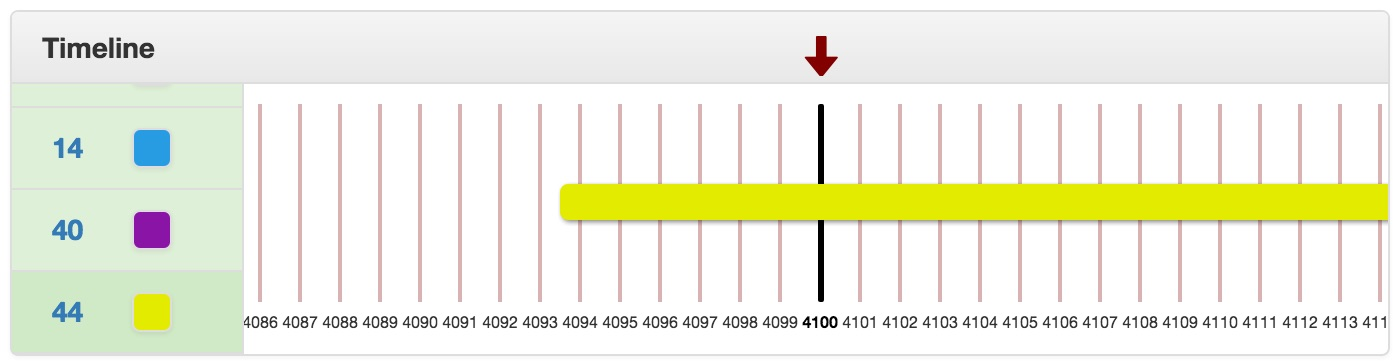
\includegraphics[scale=0.22]{images/timeline.jpg}
\end{figure}
\vspace{0.2cm}
Selecting a person in the list, the timeline displays its \textbf{history} highlighting frames where it is present. It is possible to navigate video frames by clicking on it.
\end{tframe}

\begin{tframe}{Proposals generation}
It is possible to generate \textbf{proposals} for a person in some selected frames based on previous  annotation of a it using timeline: just click and drag highlighted annotation.
\vspace{0.3cm}
Proposals generation is based on the combination of three different techniques:
\vspace{0.2cm}
\begin{itemize}
\item \textbf{Motion detection} using a \emph{background substractor}
\vspace{0.2cm}
\item \textbf{Pedestrian detection} using \emph{HOG descriptors}
\vspace{0.2cm}
\item \textbf{Kalman filter} for the \emph{motion estimation}
\end{itemize}
\end{tframe}



\end{document}